\documentclass[12pt, letterpaper]{article}
\usepackage{fullpage}
\usepackage[top=2cm, bottom=4.5cm, left=2.5cm, right=2.5cm]{geometry}
\usepackage{amsmath, amsthm, amsfonts, amssymb, amscd}
\usepackage{lastpage}
\usepackage{enumerate}
\usepackage{fancyhdr}
\usepackage{mathrsfs}
\usepackage{xcolor}
\usepackage{graphicx}
\usepackage{listings}
\usepackage{hyperref}

\hypersetup{
  colorlinks=true,
  linkcolor=blue,
  linkbordercolor={0 0 1}
}

\renewcommand\lstlistingname{Algorithm}
\renewcommand\lstlistlistingname{Algorithms}
\def\lstlistingautorefname{Alg.}

\lstdefinestyle{Python}{
    language        = Python,
    frame           = lines,
    basicstyle      = \footnotesize,
    keywordstyle    = \color{blue},
    stringstyle     = \color{green},
    commentstyle    = \color{red}\ttfamily
}

\setlength{\parindent}{0.0in}
\setlength{\parskip}{0.05in}

% Edit these as appropriate
\newcommand\course{Machine Learning}
\newcommand\hwnumber{2}                  % <-- homework number
\newcommand\NetIDa{WangZhiyi, 922182514} % <-- NetID of person #1
\newcommand\NetIDb{ZhangTianyao, 922182332} % <-- NetID of person #2 (Comment this line out for problem sets)

\pagestyle{fancyplain}
\headheight 35pt
\lhead{\NetIDa}
\lhead{\NetIDa\\\NetIDb}                 % <-- Comment this line out for problem sets (make sure you are person #1)
\chead{\textbf{\Large Homework \hwnumber}}
\rhead{\course \\ \today}
\lfoot{}
\cfoot{}
\rfoot{\small\thepage}
\headsep 1.5em


%Answer to the problem goes here.
%
%\begin{enumerate}
%  \item
%   Problem 1 part 1 answer here.
%  \item
%    Problem 1 part 2 answer here.
%
%    Here is an example typesetting mathematics in \LaTeX
%\begin{equation*}
%    X(m,n) = \left\{\begin{array}{lr}
%        x(n), & \text{for } 0\leq n\leq 1\\
%        \frac{x(n-1)}{2}, & \text{for } 0\leq n\leq 1\\
%        \log_2 \left\lceil n \right\rceil \qquad & \text{for } 0\leq n\leq 1
%        \end{array}\right\} = xy
%\end{equation*}
%
%    \item Problem 1 part 3 answer here.
%
%    Here is an example of how you can typeset algorithms.
%    There are many packages to do this in \LaTeX.
%
%    \lstset{caption={Caption for code}}
%    \lstset{label={lst:alg1}}
%    \begin{lstlisting}[style = Python]
%    from package import Class # Mesh required for..
%
%    cinstance = Class.from_obj('class.obj')
%    cinstance.go()
%    \end{lstlisting}
%
%  \item Problem 1 part 4 answer here.
%
%    Here is an example of how you can insert a figure.
%    \begin{figure}[!h]
%    \centering
%    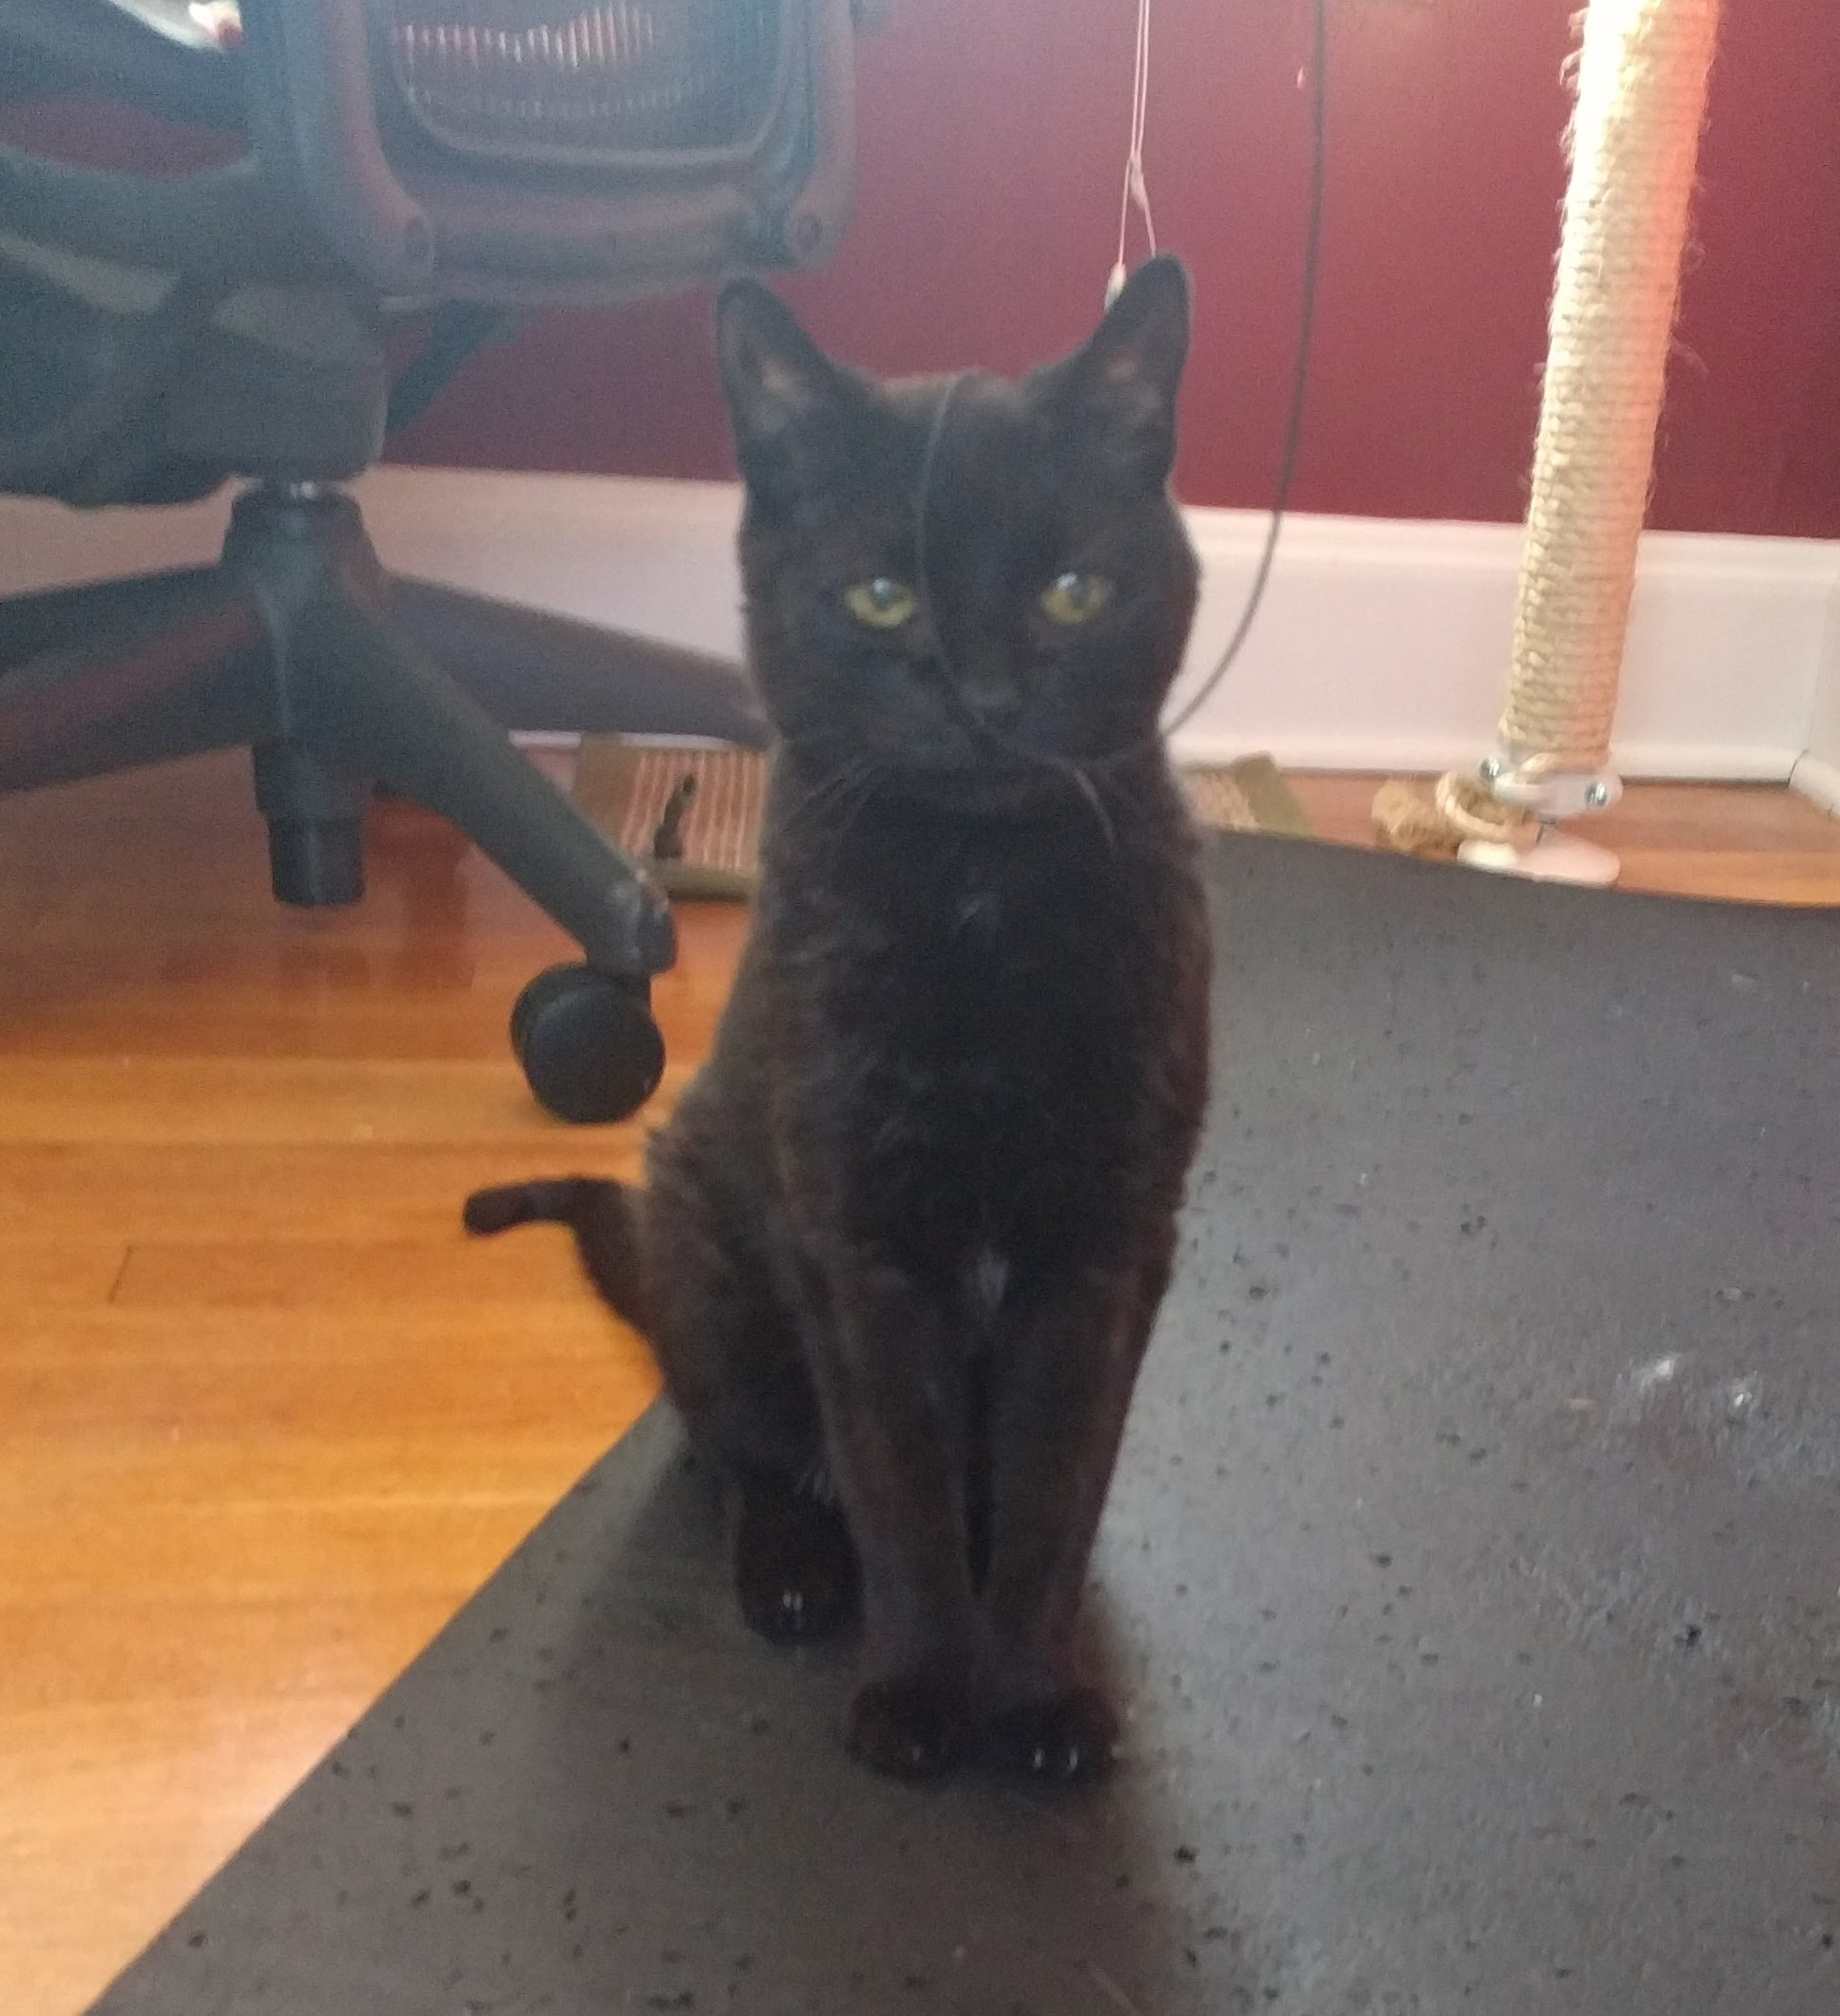
\includegraphics[width=0.3\linewidth]{heidi.jpg}
%    \caption{Heidi attacked by a string.}
%    \end{figure}
%\end{enumerate}

\begin{document}


\section*{Question 1}

\subsection*{Que (a)}
\begin{equation}
	\because A^TA=I
\end{equation}
So, $A$ is a reversible matrix.
\begin{equation}
	\Sigma_x=\frac1n\sum^6_{i=1}x_ix_i^T
\end{equation}
Among this equation, 
\begin{equation*}
\begin{align}
	x_ix_i^T
	&= Az_i(Az_i)^T\\
	&= Az_iz_i^TA^T\\
	&= A(z_iz_i^T)A^T\\
	&= AA^T
\end{align}
\end{equation*}
So that, the equation can be simplified to
\begin{equation}
\begin{align}
	\Sigma_x
	&= \frac1n\sum^6_{i=1}AA^T\\
	&= A\frac1n\sum^6_{i=1}A^T
\end{align}
\end{equation}
Then, compute the eigenvalue(s) of $\Sigma_z$
\begin{equation}
\begin{align}
	|\lambda E-\Sigma_z|
	&= \left|\begin{array}{cccc}
		\lambda-3 & 0 & 0 & 0 \\
		0 & \lambda-21 & 0 & 0 \\
		0 & 0 & \lambda-13 & -8 \\
		0 & 0 & -8 & \lambda-13 
	\end{array}\right|\\
	&= (\lambda-3)(\lambda-21)[(\lambda-13)^2-(-8)^2]\\
	&= (\lambda-3)(\lambda-21)(\lambda-21)(\lambda-5)\\
	&=0
\end{align}
\end{equation}
Solve it, we can get that
\begin{equation}
	\lambda_1=3,
	\lambda_2=21,
	\lambda_3=21,
	\lambda_4=5
\end{equation}
However, $A\in\mathbb{R}^{6\times 4}$, so we need to transform $\Sigma_x$ and $\lambda_x$
\begin{equation}
\begin{align}
	\Sigma_x
	&= AV\Lambda V^TA^T\\
	&= (AV)\Lambda (AV)^T
\end{align}
\end{equation}
Let's expand $(AV)$ to $\mathbb{R}^6$, so that
\begin{equation}
	\lambda_1=3,
	\lambda_2=21,
	\lambda_3=21,
	\lambda_4=5,
	\lambda_5=0,
	\lambda_6=0
\end{equation}
Then, compute the sum of eigenvalues
\begin{equation}
\begin{align}
	S_\lambda
	&= Tr(\Sigma_x)\\
	&= Tr(A\Sigma_zA^T)\\
	&= Tr((AA^T)\Sigma_z)\\
	&= Tr(\Sigma_z)\\
	&= 3+21+21+5+0+0\\
	&= 50
\end{align}
\end{equation}

\subsection*{Que (b)}
First, compute the estimated value of mean reconstruction error
\begin{equation}
\begin{align}
	error(d)
	&= \frac1N\sum^N_{i=1}||x_i-\tilde{x}_i||^2_2\\
	&= \sum^D_{i=d+1}\lambda_i\\
	&< \frac{50}4=17.5
\end{align}
\end{equation}
It means that
\begin{equation}
	\lambda_1+\lambda_2+\cdots+\lambda_d\geq37.5
\end{equation}
Meanwhile, sum of the top $d$ values shows that
\begin{equation}
\begin{cases}
	\max\lambda_1=21<37.5\\
	\max\lambda_1+\max\lambda_2=21+21=42>37.5
\end{cases}
\end{equation}
In conclusion, the value of PCA direction must be \textbf{not less than $2$}

\subsection*{Que (c)}
As the solving process in \textbf{Q-a} and \textbf{Q-b} above, compute the new $y$
\begin{equation}
	x\sim\mathcal{N}(0,\Sigma_x),v\sim\mathcal{N}(0,\Sigma_v)
\end{equation}
And $x$ is independent of $v$, so that
\begin{equation}
	y\triangleq x+v\in\mathcal{N}(0+0,\Sigma_x+\Sigma_v)=\mathcal{N}(0,\Sigma_x+\Sigma_v)
\end{equation}
Then compute $\Sigma_y$
\begin{equation}
\begin{align}
	\Sigma_y
	&= \Sigma_x'+\Sigma_z\\
	&= \left[\begin{array}{cccc}
		3 & 0 & 0 & 0\\
		0 & 21 & 0 & 0\\
		0 & 0 & 13 & 8\\
		0 & 0 & 8 & 13
	\end{array}\right]'+\left[\begin{array}{cccccc}
		5 & 0 & 0 & 0 & 0 & 0\\
		0 & 5 & 0 & 0 & 0 & 0\\
		0 & 0 & 5 & 0 & 0 & 0\\
		0 & 0 & 0 & 5 & 0 & 0\\
		0 & 0 & 0 & 0 & 5 & 0\\
		0 & 0 & 0 & 0 & 0 & 5
	\end{array}\right]\\
	&= \left[\begin{array}{cccccc}
		3 & 0 & 0 & 0 & 0 & 0\\
		0 & 21 & 0 & 0 & 0 & 0\\
		0 & 0 & 13 & 8 & 0 & 0\\
		0 & 0 & 8 & 13 & 0 & 0\\
		0 & 0 & 0 & 0 & 0 & 0\\
		0 & 0 & 0 & 0 & 0 & 0
	\end{array}\right]+\left[\begin{array}{cccccc}
		5 & 0 & 0 & 0 & 0 & 0\\
		0 & 5 & 0 & 0 & 0 & 0\\
		0 & 0 & 5 & 0 & 0 & 0\\
		0 & 0 & 0 & 5 & 0 & 0\\
		0 & 0 & 0 & 0 & 5 & 0\\
		0 & 0 & 0 & 0 & 0 & 5
	\end{array}\right]\\
	&= \left[\begin{array}{cccccc}
		8 & 0 & 0 & 0 & 0 & 0\\
		0 & 26 & 0 & 0 & 0 & 0\\
		0 & 0 & 18 & 8 & 0 & 0\\
		0 & 0 & 8 & 18 & 0 & 0\\
		0 & 0 & 0 & 0 & 5 & 0\\
		0 & 0 & 0 & 0 & 0 & 5
	\end{array}\right]
\end{align}
\end{equation}
\begin{equation}
\begin{align}
	|\lambda E-\Sigma_y|
	&= \left|\begin{array}{cccccc}
		\lambda'-8 & 0 & 0 & 0 & 0 & 0\\
		0 & \lambda'-26 & 0 & 0 & 0 & 0\\
		0 & 0 & \lambda'-18 & -8 & 0 & 0\\
		0 & 0 & -8 & \lambda'-18 & 0 & 0\\
		0 & 0 & 0 & 0 & \lambda'-5 & 0\\
		0 & 0 & 0 & 0 & 0 & \lambda'-5
	\end{array}\right|\\
	&= (\lambda'-8)(\lambda'-26)[(\lambda'-18)-(-8)^2](\lambda'-5)(\lambda'-5)\\
	&= (\lambda'-8)(\lambda'-26)(\lambda'-26)-(\lambda'-10)(\lambda'-5)(\lambda'-5)\\
	&= 0
\end{align}
\end{equation}
Solve it, and we get that
\begin{equation}
	\lambda_1'=8,
	\lambda_2'=26,
	\lambda_3'=26,
	\lambda_4'=10,
	\lambda_5'=5,
	\lambda_6'=5
\end{equation}
Then compute the sum of eigenvalues
\begin{equation}
\begin{align}
	S_{\lambda'}
	&= \sum^6_{i=1}\lambda'_i\\
	&= 8+26+26+10+5+5\\
	&= 80
\end{align}
\end{equation}
\begin{equation}
\begin{align}
	error'(d)
	&= \sum^D_{i=d+1}\lambda'_i\\
	&< \frac{80}4=20
\end{align}
\end{equation}
\begin{equation}
	\lambda'_1+\lambda'_2+\cdots+\lambda'_d\geq 60
\end{equation}
Meanwhile, sum of the top d values shows that
\begin{equation}
\begin{cases}
	\max\lambda'_1+\max\lambda'_2=26+26=52<60
	\max\lambda'_1+\max\lambda'_2+\max\lambda'_3=26+26+10=62>60
\end{cases}
\end{equation}
In conclusion, the new value of PCA direction must be \textbf{not less than $3$}


\section*{Question 3}

It has several options.

\begin{equation}
	\mu_x=\frac1N\sum^N_{i=1}x_i\triangleq\bar{x},\Sigma_x=\frac1N\sum^N_{i=1}(x_i-\mu_x)(x_i-\mu_x)^T
\end{equation}

\subsubsection*{Option 1}
\begin{equation}
	\mu_1(1,0),\mu_2(10^5,0)
\end{equation}
So that $\mu_1$ has all the points while $\mu_2$ has none.

\subsubsection*{Option 2}
\begin{equation}
	\mu_1(-1,0),\mu_2(2,0)
\end{equation}
So that $mu_1$ has the left point and the middle circle while $mu_2$ has the right circle.

\subsubsection*{Conclusion}
Because of this, the \textbf{Option 1} attains a lower value of the objective function.

\end{document}
